\documentclass{article}
\usepackage[utf8]{inputenc}
\usepackage{graphicx}
\usepackage{float}
\usepackage{amsmath}
\usepackage[paper=a4paper,margin=1in]{geometry}
\usepackage[table,xcdraw]{xcolor}


\title{Scale-Space Blob Detectors}
\author{David Štych\\ Aleksandra Jamróz}
\date{\today{}}



\begin{document}
\maketitle

\section{LoG filter kernel size}
Sigma is a gaussian parameter defining variance of the gaussian. In case of our task, it defines how wide the filter will spread over the image. Kernel size is dependent from chosen sigma value. Radius of kernel is in direct proportion to sigma. The bigger values, the larger blobs in the image we can detect, because the filter id wider. Meanwhile smaller sigmas allow us to find tiny blobs. That's why in order to detect blobs of all sizes, we create range of sigmas that we iterate on later.


\section{Speed comparison}
Down-sampling the image was significantly faster than changing the filter size.

\begin{table}[H]
\centering
\begin{tabular}{|
>{\columncolor[HTML]{FFFFFF}}c |c|c|}
\hline
\cellcolor[HTML]{C0C0C0}{\color[HTML]{000000} \textbf{Input image}} & \cellcolor[HTML]{C0C0C0}{\color[HTML]{000000} \textbf{\begin{tabular}[c]{@{}c@{}}Time {[}ms{]}\\ changing filter size\end{tabular}}} & \cellcolor[HTML]{C0C0C0}{\color[HTML]{000000} \textbf{\begin{tabular}[c]{@{}c@{}}Time{[}ms{]}\\ down-sampling the image\end{tabular}}} \\ \hline
{\color[HTML]{000000} sunflowers.jpg}                               & {\color[HTML]{000000} 247.194}                                                                                                       & {\color[HTML]{000000} 104.404}                                                                                                         \\ \hline
{\color[HTML]{000000} fruits.jpg}                                   & {\color[HTML]{000000} 359.280}                                                                                                       & {\color[HTML]{000000} 136.804}                                                                                                         \\ \hline
{\color[HTML]{000000} water\_texture.jpg}                           & {\color[HTML]{000000} 302.661}                                                                                                       & {\color[HTML]{000000} 139.446}                                                                                                         \\ \hline
\end{tabular}
\end{table}


Down-sampling the image takes some processing time. However, after it is done, all subsequent convolution operations are simplified and require less time to complete. We noted over 2x improvement of results after using down-sampling algorithm instead of the changing filter size one. 

\section{Scale-space selection}
Our parameters are:
\begin{align*}
\sigma_0&=\frac{R_{min}}{\sqrt{2}}=\frac{2}{\sqrt{2}}\\
s&=[1.2,  1.6] \quad  \textit{We tuned the parameter to obtain desired results.}\\
k&=0,1,2...9
\end{align*}
We chose $\sigma_0$ value depending on the smallest predicted blob radius, marked as $R_{min}$. Next sigmas are calculated according to the given equation:
\begin{align*}
\sigma_k = \sigma_0s^k 
\end{align*}


\section{Down-sampling image - scale}
We selected $\sigma_0$ the same way $\sigma_0=\frac{R_{min}}{\sqrt{2}}$.
The image is then scalled down with factor $s^k$, while keeping $\sigma$ constant $\sigma=\sigma_0$.

In the first iteration, the scale is not changed $s^0$.

\section{Down-sampling image - normalization}
As $\sigma$ increases, derivatives are attenuated. We need to normalize the filter response by multiplying it by $\sigma^2$.

However, when down-sampling the image, we keep $\sigma$ constant. Therefore, it is not necessary to normalize the filter response.



\section{Non-maximum suppresion function}

\begin{figure}[H]
\centering
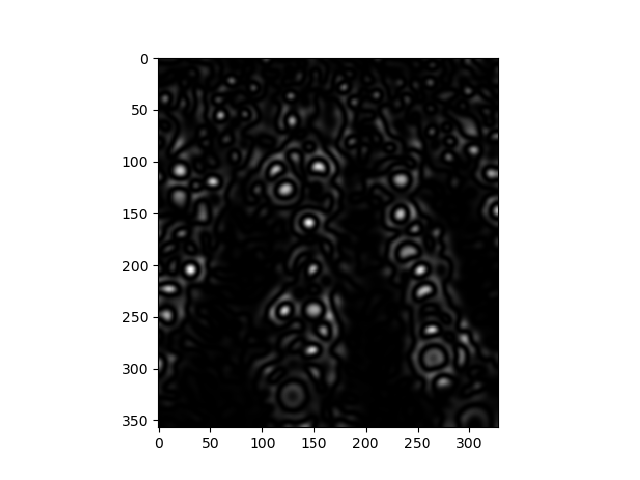
\includegraphics[width=0.8\textwidth]{figs/filter_response.png}
\caption{Filter response}
\label{fig:filter_resp}
\end{figure}
Figure \ref{fig:filter_resp} shows the filter response. The goal of the non-maximum suppression function is to find the local maxima of the filter response. As we see on the image, we try to separate white regions from black background. Some blobs are filtered using thresholds. Overlapping blobs are removed as well.


\section{Other images}
By default, the LoG filter looks for dark blobs.
\vspace*{0.3cm}

For image \textit{sunflowers.jpg} we squared the filter response. It is because we are looking for dark as well as light blobs. Therefore, squaring the filter response makes it positive everywhere and we can find dark/light blobs based on the amplitude.
\begin{verbatim}
filtered = ndimage.gaussian_laplace(image, sigma=s)**2
\end{verbatim}

\vspace*{0.4cm}
For image \textit{water\_texture.jpg} we kept the original filter (no changes in sign or squaring the response). It is because we are looking for dark blobs only. 
\begin{verbatim}
filtered = ndimage.gaussian_laplace(image, sigma=s)
\end{verbatim}

\vspace*{0.4cm}
For image \textit{fruits.jpg} we multiplied the filter response by -1. It is because we are looking for light blobs only.
\begin{verbatim}
filtered = -ndimage.gaussian_laplace(image, sigma=s)
\end{verbatim}     

\newpage
\section{Sample images}
\begin{figure}[H]
\centering
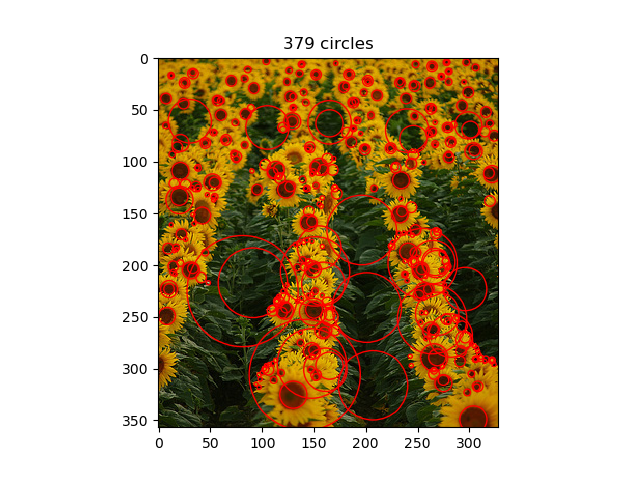
\includegraphics[width=0.8\textwidth]{figs/sunflowers_filter.png}
\caption{\textit{sunflowers.jpg} processed by changing filter size}
\end{figure}


\begin{figure}[H]
\centering
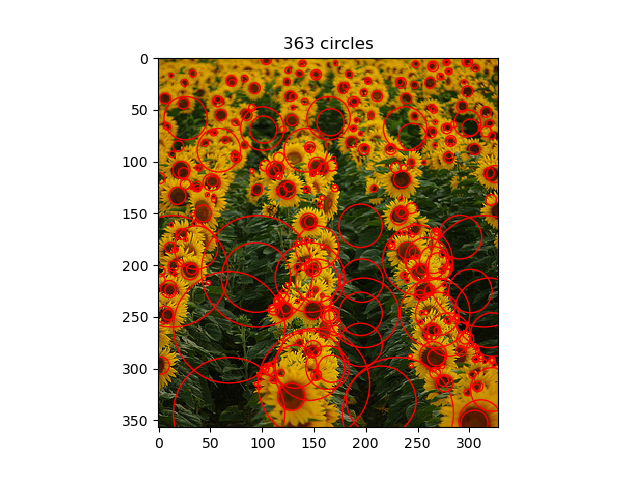
\includegraphics[width=0.8\textwidth]{figs/sunflowers_image.png}
\caption{\textit{sunflowers.jpg} processed by changing image size}
\end{figure}



\begin{figure}[H]
\centering
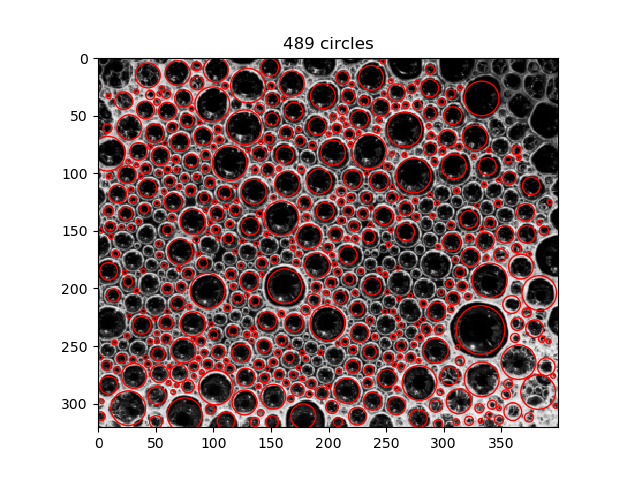
\includegraphics[width=0.8\textwidth]{figs/water_filter.png}
\caption{\textit{water\_texture.jpg} processed by changing filter size}
\end{figure}



\begin{figure}[H]
\centering
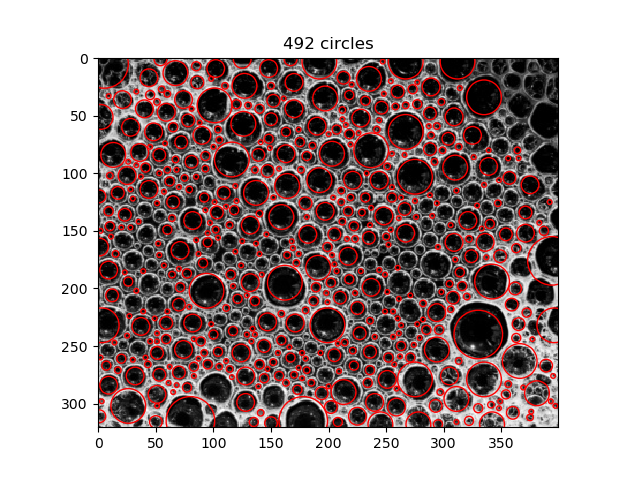
\includegraphics[width=0.8\textwidth]{figs/water_image.png}
\caption{\textit{water\_texture.jpg} processed by changing image size}
\end{figure}



\begin{figure}[H]
\centering
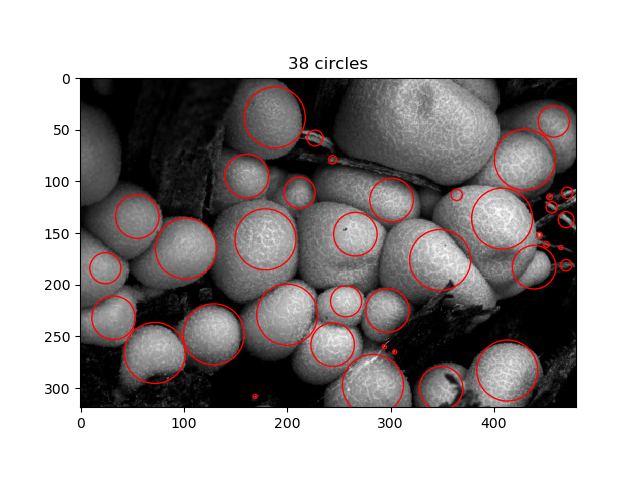
\includegraphics[width=0.8\textwidth]{figs/fruits_filter.png}
\caption{\textit{fruits.jpg} processed by changing filter size}
\end{figure}



\begin{figure}[H]
\centering
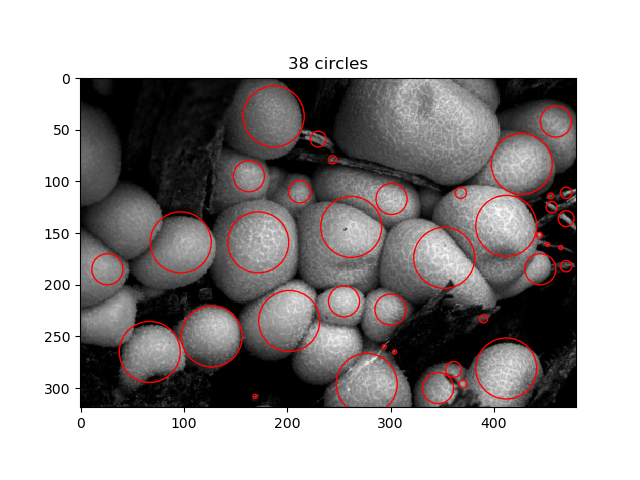
\includegraphics[width=0.8\textwidth]{figs/fruits_image.png}
\caption{\textit{fruits.jpg} processed by changing image size}
\end{figure}




\end{document}





